\section{Разработка программного средства} 
\label{sec:development}

Для реализации программного средства использовался Webix -- JavaScript библиотека, разработанная специально для работы с UI.

Инструменты, предоставляемые данной библиотекой, позволяют быстрее разрабатывать веб-приложения благодаря широкому набору готовых <<умных>> компонентов с богатым набором предоставляемых свойств и методов.

Список компонентов, созданных с целью предоставления пользователю интерфейса для взаимодействия с программным средством, предоставляемых библиотекой Webix, представлен на рисунке~\ref{sec:development:webix_control_widgets}.

\begin{figure}[ht]
  \centering
    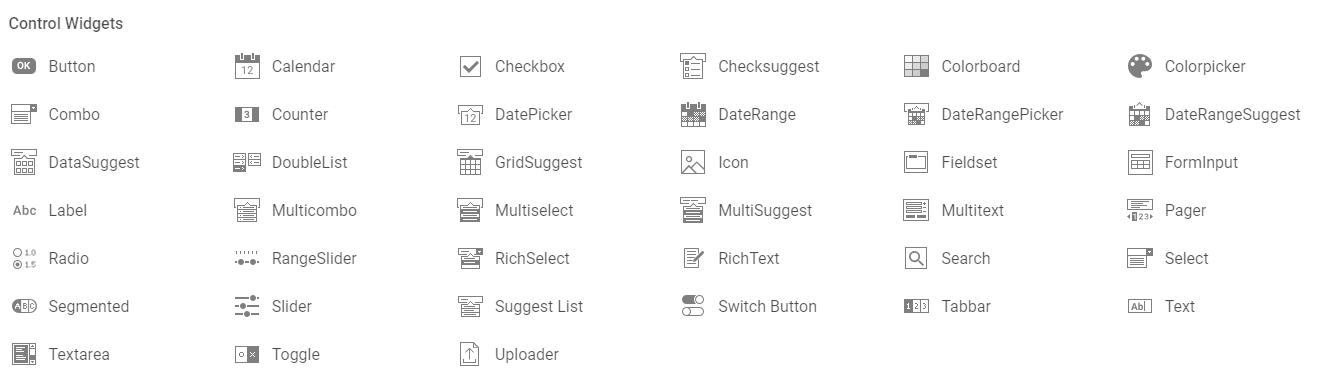
\includegraphics[scale=0.47]{webix_control_widgets.png}
    \caption{Список комплексных Webix-компонентов, способных работать с наборами данных}
    \label{sec:development:webix_control_widgets}
\end{figure}

Список компонентов, способных работать с наборами данных, предоставляемый библиотекой Webix представлен на рисунке~\ref{sec:development:webix_data_widgets}.

\begin{figure}[ht]
  \centering
    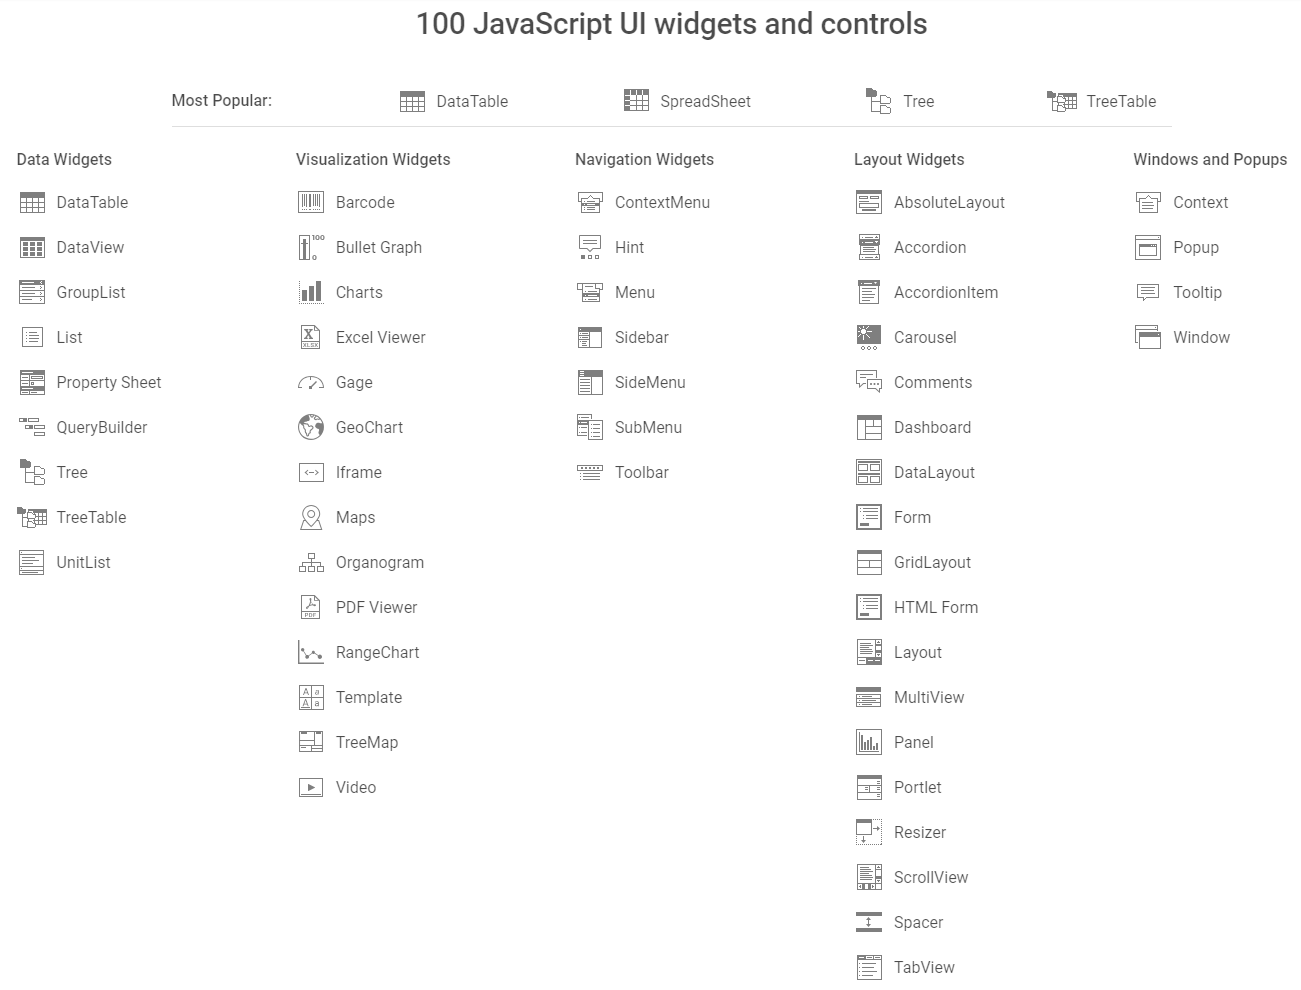
\includegraphics[scale=0.47]{webix_data_widgets.png}
    \caption{Список комплексных Webix-компонентов, способных работать с наборами данных}
    \label{sec:development:webix_data_widgets}
\end{figure}

Предоставляемое разнообразие готовых ui компонентов позволит создавать пользователям виджеты разной сложности под собственные нужды. \pagebreak

Основная функциональность программного средства заключена в трех главных компонентах: 
\begin{itemize}
	\item палитра компонентов -- панель, где отображается список доступных компонентов и пресетов, доступных пользователю, и именно отсюда осуществляется перетягивание компонентов на грид;
	\item грид -- разметка, куда осуществляется <<бросание>> компонентов пользователем;
	\item инспектор свойств -- панель, созданная для редактирования свойств компонентов, содержит все необходимые инструменты, чтобы определить то, как будет работать компонент.
\end{itemize}
  
На рисунке~\ref{sec:development:schema_classes} представлена диаграмма классов графических компонентов типа <<layout>>, представленных в приложении. Список классов может пополняться в результате расширения приложения разработчиками.\pagebreak

\begin{figure}[ht]
  \centering
    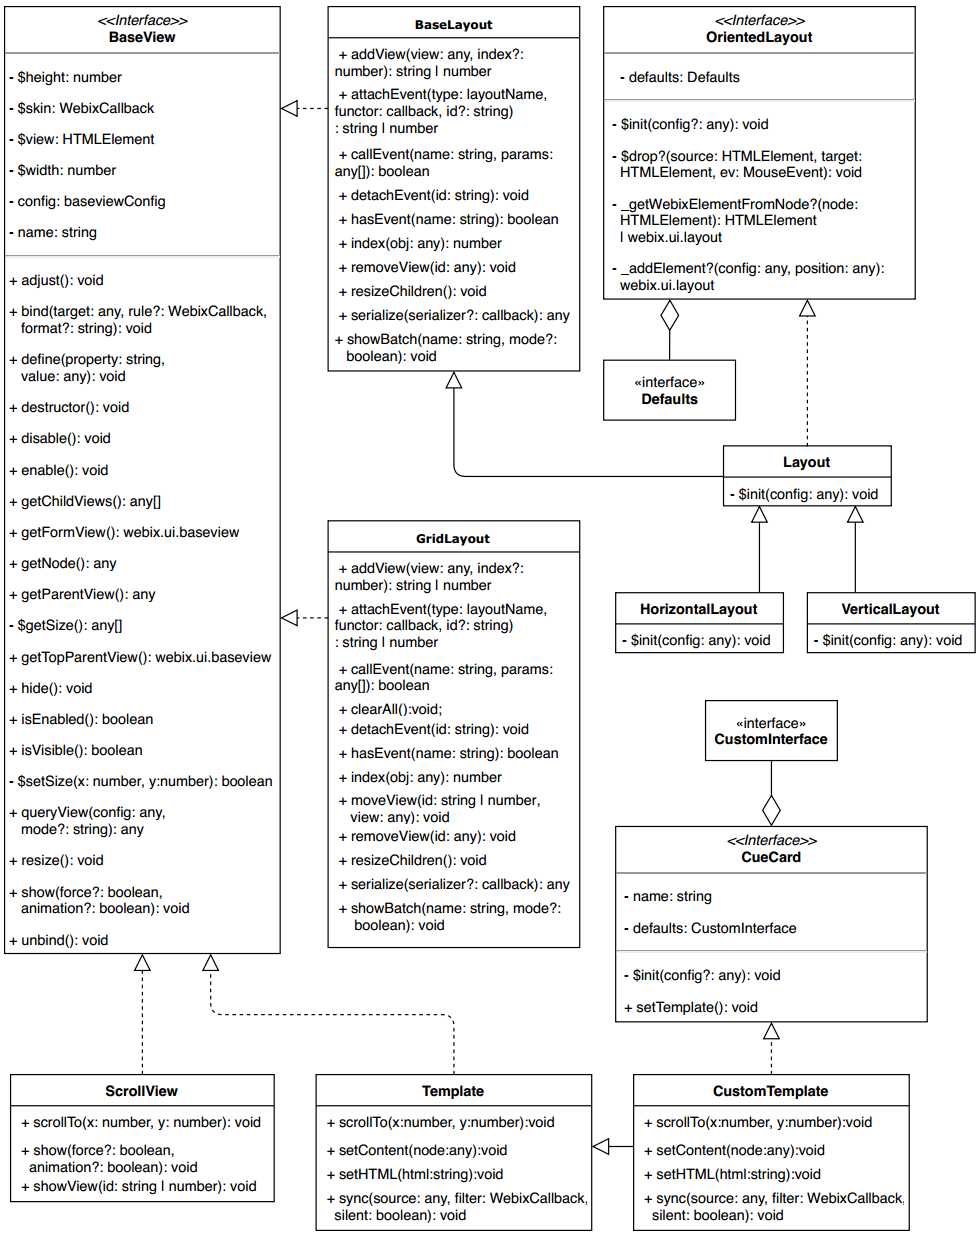
\includegraphics[scale=0.57]{schema_classes.png}
    \caption{Диаграмма классов программного средства}
    \label{sec:development:schema_classes}
\end{figure}

\subsection{Cборщик проекта}
\label{sec:development:bundler}

Инструменты сборки стали неотъемлемой частью веб-разработки, в основном из-за возрастающей сложности JS-приложений. Бандлеры позволяют нам упаковывать, компилировать, организовывать множество ресурсов и библиотек, необходимых для современного веб-проекта.

В ходе процесса разработки в качестве сборщика проекта был использован Webpack.

Webpack - сборщик проекта, который помогает автоматизировать второстепенные задачи веб-разработки и чаще всего используется для оперирования файлами и папками внутри проекта, преобразования таблиц стилей, написанных с применением синтаксиса SASS, LESS и др. в формат стандартных таблиц стилей CSS. Его также часто используют для выполнения задачи минификации кода проекта при помощи специальных плагинов – оптимизации в один или несколько файлов, что исключительно положительно сказывается на конечной производительности проекта.

Помимо этого, Webpack может путем анализа кода проекта удалять из него неиспользуемые части, что может привести к значительному уменьшению минифицированного варианта проекта. Из всего вышесказанного можно сделать вывод о том, что Webpack – мощный инструмент, который существенно облегчает процесс разработки проекта.

Webpack, мощный бандлер с открытым исходным кодом, который может обрабатывать огромное количество различных задач и является одним из самых мощных и гибких инструментов для сборки frontend. 

Плюсы:

\begin{itemize}
    \item великолепен для работы с одностраничными приложениями;
    \item воспринимает как require()- так и import-синтаксисы модуля;
    \item позволяет осуществлять продвинутое разделение кода;
    \item hot reload для более быстрой разработки с помощью React, Vue.js и подобных  фреймворков;
    \item наиболее популярный инструмент разработки по версии обзора JS в 2016 году.
\end{itemize}

Минусы:

\begin{itemize}
    \item не подойдет для новичков;
    \item работа с файлами CSS, картинками и другими не JS ресурсами по началу сбивает с толку;
    \item очень много изменений, большинство гайдов 2016 уже устарели;
\end{itemize}

\subsection{Среда разработки Visual Studio Code}
\label{sec:development:ide}

Visual Studio Code — программное средство, разработанный Microsoft для Windows, Linux и macOS. Позиционируется как «лёгкий» редактор кода для кроссплатформенной разработки веб- и облачных приложений. Включает в себя отладчик, инструменты для работы с Git, подсветку синтаксиса, IntelliSense и средства для рефакторинга. Имеет широкие возможности для кастомизации: пользовательские темы, сочетания клавиш и файлы конфигурации. 

Распространяется бесплатно, разрабатывается как программное обеспечение с открытым исходным кодом, но готовые сборки распространяются под проприетарной лицензией.

Visual Studio Code основан на Electron — фреймворк, позволяющий с использованием Node.js разрабатывать настольные приложения, которые работают на движке Blink. Несмотря на то, что редактор основан на Electron, он не использует редактор Atom. Вместо него реализуется веб-редактор Monaco,разработанный для Visual Studio Online.

Visual Studio Code — это редактор исходного кода. Он поддерживает ряд языков программирования, подсветку синтаксиса, IntelliSense, рефакторинг, отладку, навигацию по коду, поддержку Git и другие возможности. Многие возможности Visual Studio Code не доступны через графический интерфейс, зачастую они используются через палитру команд или JSON файлы (например, пользовательские настройки). Палитра команд представляет собой подобие командной строки, которая вызывается сочетанием клавиш.

Visual Studio также позволяет заменять кодовую страницу при сохранении документа, символы перевода строки и язык программирования текущего документа.

С 2018 года появилось расширение Python для Visual Studio Code с открытым исходным кодом. Оно предоставляет разработчикам широкие возможности для редактирования, отладки и тестирования кода.

На март 2019 года посредством встроенного в продукт пользовательского интерфейса можно загрузить и установить несколько тысяч расширений только в категории «programming languages» (языки программирования).
\subsection{Описание структуры приложения}
\label{sec:development:app_structure}

На рисунке~\ref{sec:development:app_structure_pic} представлена файловая структура проекта, который является клиентским приложением.

Проект состоит из следующих основных частей:

\begin{itemize}
    \item папка Components, содержащая исходный код компонентов;
    \item папка helpers, содержащая некторые часто применяемые участки кода, вынесенные в отдельные функции;
    \item папка styles, содержащая CSS-стили для всего проекта.
\end{itemize}

Папка Components в свою очередь включает в себя все существующие компоненты и состоит из:

\begin{itemize}
    \item папка componentsPallet, содержащая исходный код палитры компонентов;
    \item папка componentsLayout, содержащая исходный код грида;
    \item папка cueCards, содержащая исходный код пользовательских шаблонов;
    \item папка layouts, содержащая исходный код основных предоставляемых компонентов;
    \item папка propertyInspector, содержащая исходный код инспектора свойств.
\end{itemize}

Папка layouts, как уже было сказано выше, включает в себя папки, содержащие исходный код каждого из присутствующих в программном компонентов. Этими папками являются:

\begin{itemize}
    \item папка baselayout содержит исходный базового компонента, чья функциональность используется во всех компоненах типа <<layout>>;
    \item папка gridlayout, содержит исходный особого компонента типа <<layout>>, который использует совершенно другой способ позиционироваия дочерних элементов, нежели baselayout: в отличие от последнего, где используется смещение в пикселях от левой верхней точки, здесь используется абсолютное позиционирование по виртуальным клеткам;
    \item папка helpers, содержащая некторые часто применяемые в компонентах участки кода, вынесенные в отдельные функции;
    \item папки horizontal layout и vertical layout содержат исходный код одноименных компонентов, осуществояющих позиционирование дочерних компонентов либо в колонки (горизонтально), либо в строки (вертикально).
\end{itemize}

\begin{figure}[ht]
\centering
    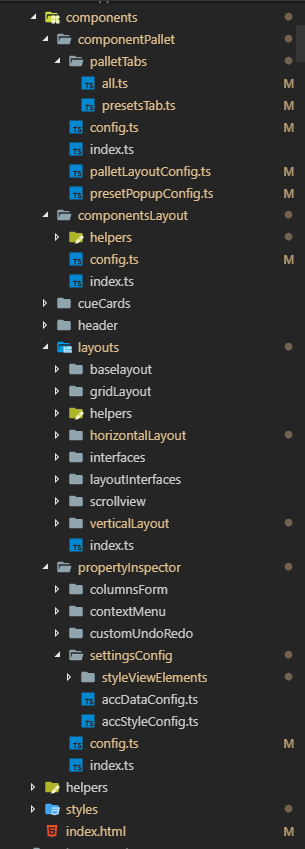
\includegraphics[scale=0.6]{app_structure.png}
    \caption{Файловая структура проекта}
    \label{sec:development:app_structure_pic}
\end{figure}
    
\subsection{Разработка палитры компонентов}
\label{sec:development:component_palett}

Для инициализации компонента палитры были использованы компоненты библиотеки Webix. Для отображения разных вкладок на панели использвался компонент TabView, а для отображения данных и источника <<перетягивания>> комопннетов использовался компонент DataView, так как имеет встроенные возможности для работы с алгоритмом Drag-n-drop. 

\subsubsection{}Способ предсоставления компонентов
\

Каждой вкладке соответствует свой DataView, отображающий дозированные согласно названию вкладки данные, управляет отображением же TabView. Далее будет представлен основной код палитры компонентов.

\begin{lstlisting}
import getAllTabConfig from './palletTabs/all';
import { getPresetsTabConfig } from './palletTabs/presetsTab';

const getDefaultComponentPalletLayout = dataContent => ({
  rows: [
    {
      view: 'search',
      placeholder: 'Search 1,000,000 images...'
    },
    {
      view: 'tabview',
      cells: [
        {
          header: 'All',
          body: getAllTabConfig(dataContent)
        },
        {
          header: 'Presets',
          body: getPresetsTabConfig()
        },
        ...componentContainers(dataContent)
      ]
    }
  ]
});
\end{lstlisting}

Содержимое массива, возвращаемого функцией componentContainers являются DataView компоненты, каждый и который соответствует сожержанием своей вкладке.

\begin{lstlisting}
const DATAVIEW_TEMPLATE = '<span class="webix-icon fa fa-#icon#"></span>  #element#';
const LAYOUT_DATAVIEW_CONFIG = 'pallet:dataview:layouts';
const COMPONENTS_DATAVIEW_CONFIG = 'pallet:dataview:components';
const CUECARDS_DATAVIEW_CONFIG = 'pallet:dataview:cuecards';

const componentContainers = data => [{
  header: 'Layouts',
  body: {
    view: 'dataview',
    template: DATAVIEW_TEMPLATE,
    id: LAYOUT_DATAVIEW_CONFIG,
    xCount: 3,
    drag: 'source',
    minHeight: 200,
    data: data.layouts
  }
},
{
  header: 'Components',
  body: {
    view: 'dataview',
    template: DATAVIEW_TEMPLATE,
    id: COMPONENTS_DATAVIEW_CONFIG,
    xCount: 3,
    drag: 'source',
    minHeight: 200,
    data: data.components
  }
},
{
  header: 'Cue cards',
  body: {
    view: 'dataview',
    template: DATAVIEW_TEMPLATE,
    id: CUECARDS_DATAVIEW_CONFIG,
    xCount: 3,
    drag: 'source',
    minHeight: 200,
    data: data.templates.map(element => ({
      ...element,
      template: element.template
    }))
  }
}]
\end{lstlisting}

Каждый DataView компонент отвечает за отображение своей части данных, а указание свойства <<drag: 'source' предоставляет возможность использовать компонент как источник данных (пункта <<тащи>> или <<drag>>) для реализации алгоритма Drag-n-drop.

Объект конфигураций самого компонента выглядит следующим образом:

\begin{lstlisting}
import getDefaultComponentPalletLayout from './palletLayoutConfig';
import { onPresetLoad } from './palletTabs/presetsTab';
import ComponentPallet from '../layouts/interfaces/ComponentPallet';

const componentPalletConfig: ComponentPallet = {
  name: 'AppOrchid-Component-Pallet',
  defaults: {
    // defaults here

  },
  $init() {
    // initialization here
  },
  _getComponentViewConfig() {
    if (!this.config.componentView || typeof this.config.componentView !== 'object') {
      return this.config.defaultComponentView;
    }

    return this.config.componentView;
  },
  _getComponentView() {
    return this.queryView({ ...this.config.defaultComponentView });
  }
};
\end{lstlisting}

Загрузка содержимого DataView компонентов - преопределенных конфигураций графических компонентов, осуществляется самим Component-Pallet при его инициализации путем, регламентированным библиотекой Webix.

\begin{lstlisting}
$init() {
  this.$ready.push(
    () => {
    webix.ajax().get(this.config.widgets)
      .then(res => res.json())
      .then(res => ({
        layouts: res.layouts.map(item => ({ ...item, widgetType: 'layout' }),
        components: res.components.map(item => ({ ...item, widgetType:'component' })),
        templates: res.templates.map(item => ({ ...item, widgetType: 'card'}))
      }))
      .then((res) => {
        this.addView({
          ...getDefaultComponentPalletLayout(res)
        });
      })
      .catch((e) => {
        console.error(e);
      });
    },
    () => {
      if (!this.config.gridId) { return; }
      let loadPreset = onPresetLoad.bind(this);
      this.attachEvent('onPresetLoad', loadPreset);
    }
  );
}
\end{lstlisting}

Применение кастомной конфигурации к базовому компоненту осуществляется путем применения метода protoUI глобального объекта webix к конфигурации нашего компонента Component-Pallet и базовым классам, предоставляемым библиотекой Webix:
\begin{itemize}
    \item webix.IdSpace - для изоляции содержимого;
    \item webix.ui.layout - для доступа к функциональности базового лэйаута.
\end{itemize}

\begin{lstlisting}
webix.protoUI(
  componentPalletConfig,
  webix.IdSpace,
  webix.ui.layout
);
\end{lstlisting}

По умолчанию предполагается, что в получаемом в результате запроса JavaScript-объекте должны быть поля: layouts, components и card - три вида лэйаутов. Однако, эти параметры могут быть изменены разработчиком, интегрирующим данное програмнное средство в свой проект.

\subsubsection{}Пресеты
\

В палитре компонентов, как указывалось ранее, доступна возможность загрузки и применения пресетов - предопределенных наборов компонентов, которые были созданы и предоставлены разработчиками или, например, другими пользователями.

Доступ к пресетам осуществляется через соответствующую вкладку <<Presets>>. Лист пресетов получает их конфигурации из объекта, реализующего доступ к данным в библиотеке Webix - DataCollection.

\begin{lstlisting}
{
  id: getPresetsListId(),
  borderless: true,
  data: webix.storage.local.get('collection') || [{ name: 'No presetsfound' }],
  view: 'list',
  select: true,
  template: `#name#${DELETE_PRESET_ICON_TEMPLATE}`,
  on: {
      onItemDblClick(id): void {
      const topParent = this.getTopParentView();
      topParent.callEvent('onPresetLoad', [this.getItem(id)]);
      }
  },
  onClick: {
    'fa-trash-o': function (ev, id): void {
      const self = this;
      webix.confirm({
        text: 'Item data will be lost. <br/> Are you sure?',
        ok: 'Yes',
        cancel: 'Cancel',
        callback: (res) => {
          removePreset.apply(self, [res, id]);
        }
      });
    }
  }
}
\end{lstlisting}

Сохранение текущей конфигурации осуществляется путем сериализации содержимого грида. Для этого вызывается метод объекта грида getSerializedCollection, логика которого будет рассмотрена позднее.

\begin{lstlisting}
const topParent = $$(this.getTopParentView().config.master)
.getTopParentView();

const gridId = $$((topParent.config).gridId);

const newElement = savePreset(this.getValue(), $$(gridId)
  .getSerializedCollection());
this.getTopParentView().hide();

if (newElement) {
  topParent.$$(getPresetsListId()).parse(newElement);
}
\end{lstlisting}

Применение пресета из списка доступных осуществляется в несколько этапов. 
Первым является вызов события onPresetLoad, на срабатывание которого вызывается колбэк с соответствующим именем, в котором осуществляется первичная проверка данных и дальнейшая делегация выполнения применения пресета.

\begin{lstlisting}
function onPresetLoad(preset) {
  const grid = ($$(this.config.gridId));

  if (preset.content) {
    let arr = $$(this.config.gridId)
      .getChildViews();

    for (let i = arr.length - 1; i > 0; i--) {
      grid.removeView(arr[i]);
    }

    webix.delay(() => {
      loadPreset(preset.content, grid);
    });

    webix.message({
      text: `Preset ${preset.name} loaded`,
      expire: 1000
    });
  } else {
    webix.message({
      text: 'No data provided',
      type: 'error'
    });
  }
}
\end{lstlisting}

Вызываемая внутри функция loadPreset вызывает функцию saveAndRender для каждого объекта, которому соответствует компонент.

\begin{lstlisting}  
const loadPreset = (collection: object, grid: ComponentsLayout)=> {
  Object.keys(collection)
    .forEach((presetId) => {
    saveAndRender(collection[presetId], grid);
  });
};    
\end{lstlisting}

Метод saveAndRender в свою очередь добавляет нужные позиционные свойства компонентам, которые будут помещаться на грид и вызывает у грида метод рендера. В качестве параметра туда передается конфиг компонента и его будущие координаты.

\begin{lstlisting}
    
const saveAndRender = (source: any, grid: ComponentsLayout) => {
  const id = webix.uid();
  let item = { id, ...source };
  
  if (!item.parentId) {
    const width = item.width || 0;
    const height = item.height || 0;
  
    const offsetX = Number(item.left + (width / 2));
    const offsetY = Number(item.top + (height / 2));
  
    grid._addMovableElement(item, {
      offsetX,
      offsetY
    });
  }
  return item;
};
\end{lstlisting}

Удаление пресета из списка осуществляется путем удаления пресета из коллекции, к которой <<привязан>> список пресетов. Путем простой фильтрации по условию неравенства уникальному свойству удаляемого пресета и осуществляется процесс удаления.

\begin{lstlisting}
function removePreset(result: any, id: string | number) {
  if (result) {
    let presetsCollection = webix.storage.local.get('collection');
    if (!presetsCollection || !presetsCollection.length) {
      return;
    }
    presetsCollection.filter(element => element.name !== this.getItem(id).name);

    this.remove(id);

    webix.storage.local.put('collection', presetsCollection);
  }
}
\end{lstlisting}

Резюмируя, можно сделать вывод, что был разработан гибкий инструмент для использования предопределенных наборов компонентов, предоставляющий функциональность как добавления и применения пресетов, так и их удаления.
\subsection{Разработка грида}
\label{sec:development:grid}

Грид выступает инструментом для отображения компонентов, перетянутых с палитры компонентов. Это основной компонент, занимающий большую часть экрана. Он представляет собой разметку с сеткой, размер которой может быть изменен.

\subsubsection{Алгоритм Drag-n-drop}
\

Создание и перемещение компонентов осуществляется методами, реализующими алгоритм Drag-n-drop. Для этого был разработан объект Movable, методы которого предоставлет методы $\$$dragCreate, $\$$dragPos и $\$$dragDestroy.

Метод $\$$dragCreate отвечает за начало перетягивания компонента. Библиотека Webix предполагает наличие метода с таким названием и выполнение им строго определенных функций, в частности, если начинает перетягиватся компонент, возвращать его DOM-элемент, иначе - false.

\begin{lstlisting}
$dragCreate(object, e) {
  let master = webix.DragControl.getMaster(object).master;

  if ($$(e.target.getAttribute('view_id')) &&
    $$(e.target.getAttribute('view_id')).config.view === 'resizer') {
    return false;
  }

  if (master.config.move) {
    let offset = webix.html.offset(object);
    let pos = webix.html.pos(e);

    webix.DragControl.top = offset.y - pos.y;
    webix.DragControl.left = offset.x - pos.x;
    return webix.toNode(master.$view);
  }
  return false;
}
\end{lstlisting}

Метод $\$$dragDestroy осуществляет финализацию процесса перетягивания компонента: очистку используемых ресурсов, убирание тени от движения компонента, вызов события окончания движения и т.д.

\begin{lstlisting}
$dragDestroy() {
  const master = this.master.getChildViews()[0.$view.getBoundingClientRect();
  const grid = this.master.getParentView();

  const gridBounds = this.master.getParentView()
    .$view
    .getBoundingClientRect();
  let view = this.master;

  let diffX = master.x - gridBounds.x;
  let diffY = master.y - gridBounds.y;

  let { left, top } = stickToGrid(this.master,diffX, diffY, grid.config.separation);

  if (view._settings) {
    view._settings.top = top + 7;
    view._settings.left = left + 7;
  }

  webix.DragControl.top = 5;
  webix.DragControl.left = 5;

  view.resize();

  removeShadow();

  this.master.callEvent('onViewMoveEnd', []);
  let item = this.master.getChildViews()[0];

  item.config.top = this.master.config.top;
  item.config.left = this.master.config.left;

  const elem = view.getChildViews()[0];

  elem.callEvent('onBlur', []);
  elem.callEvent('onFocus', [elem]);
}
\end{lstlisting}

Метод $\$$dragPos отвечает за перерисовку компонента и грида во время движения первого. 

\begin{lstlisting}
$dragPos(pos, e) {
  this.master.callEvent('onViewMove', [pos, e]);

  const grid = this.master.getParentView();
  const gridBounds = grid.$view.getBoundingClientRec();

  let context = webix.DragControl.getContext();
  let control = context.source;

  pos.x = e.clientX - gridBounds.x;
  control.style.left = pos.x;
  pos.y = e.clientY - gridBounds.y;
  control.style.top = pos.y;

  const master = this.master.getChildViews()[0.$view.getBoundingClientRect();

  let diffX = master.left - gridBounds.x;
  let diffY = master.top - gridBounds.y;

  let { left, top } = stickToGrid(this.master, diffX, diffY, grid.config.separation);

  let shadowRect = document.getElementsByClassNam('element-shadow')[0];

  if (shadowRect) {
    removeShadow();
  }

  if (!shadowRect
    || (shadowRect.getBoundingClientRect().left !== left
    && shadowRect.getBoundingClientRect().top !== top)) {
      drawShadow(this.master.$view, left + 10, top + 10, grid.getNode());
  }
}
\end{lstlisting}

\subsubsection{Разработка сетки грида и реализация <<магнитной привязки>>}
\

Сетка грида выполняет не только декоративную функцию и несколько упрощает визуальное выравнивание компонентов, но и обладает свойством магнитной привязки. Алгоритм отрисовки сетки представлен ниже.

\begin{lstlisting}
drawCanvasGrid() {
  const self = this;
  const conf = {
    template: () => `<canvas
      id ="${self._canvasId}"
      height="${document.body.clientHeight}"
      width="${document.body.clientWidth}"
    />`,

    top: 0,
    left: 0,
    zIndex: -10,

    autoheight: true,
    presetParse: false,
    
    on: {
        onAfterRender() {
            this.define('height', document.body.clientHeight);
            this.define('width', document.body.clientWidth);
            this.resize();

            self._drawGrid();
        }
    }
  };
  this.addView(conf);
}
\end{lstlisting}

Данный алгоритм предоставлет возможность редактировать размер сетки, суть которой заключается в том, что компоненты можно передвигать лишь с шагом, равным размеру клетки в пикселях. Вызовы метода stickToGrid выполняют дополнительные высчитывания координат места, куда будет позиционирован перетягиваемый компонент по окончании.

Также помимо сетки, присутствует тень от компонента, которая показывает, куда компонент будет помещен, когда пользователь отпустит нажатую для перетягивания компонента левую кнопку мыши или уберет палец от сенсорного экрана.

Алгоритм рисования тени предполагает вызов перерисовки тени на каждое событие движения мыши.

\begin{lstlisting}
const drawShadow = (htmlView, left, top, grid) => {
  const shadow = document.createElement('div');

  const viewRect = htmlView.children[0.getBoundingClientRect();
  shadow.className = 'element-shadow';

  shadow.style.top = `${top}px`;
  shadow.style.left = `${left}px`;
  shadow.style.width = `${viewRect.width - 1}px`;
  shadow.style.height = `${viewRect.height - 1}px`;
  shadow.style.position = 'relative';

  grid.appendChild(shadow);
}

const removeShadowGrid = () => {
  let div = document.getElementsByClassName('grid-shadow')[0];
  div.parentNode.removeChild(div);
};
\end{lstlisting}

Добавление функицональности Drag-n-drop осуществляется путем вызова метода addDrop объекта DragControl, который доступен через глобальный объект webix.
Вызов метода происходит в методе инициализации грида $\$$init.

\begin{lstlisting}
webix.DragControl.addDrop(self.$view, {
  $drop(source, target, ev) {
    let dnd = webix.DragControl.getContext();

    if (dnd.from.name === 'dataview' &&
      (dnd.from.getItem(dnd.source[0]).widgetType === 'layout' ||dnd.from.getItem(dnd.source[0]).widgetType === 'card')
    ) {
        if (dnd.from.name === 'dataview') {
          let elementConfig = webix.copy(dnd.from.getItem(dnd.source[0].config);

          if (elementConfig.view === 'AppOrchid-Gridlayout') {
            self._onGridLayoutDrop(elementConfig, ev);
            return;
          }

          elementConfig.id = webix.uid();
          self._addMovableElement(elementConfig, ev);
        }
    } else if (dnd.from.name === 'dataview' && 
    dnd.from.getItem(dnd.source[0]).widgetType !== 'layout') {
      webix.message({
        text: 'Only layouts can be placed on the grid',
        type: 'error',
        expire: 2000
      });
    }
  }
})
\end{lstlisting}

Добавление элемента на грид осуществляется методом внутренним приватным методом $\_$addMovableElement, который добавляет внутренние свойства к конфигу компонента, необходимые для дальнейшей работы.

\begin{lstlisting}
_addMovableElement(config, ev) {
  let height;
  let width;
  let top;
  let left;
  const self = this;

  // when vertical or horizontal layout
  if (!config.width || !config.height) {
    width = this.config.separation;
    height = this.config.separation;
  } else {
    width = config.width;
    height = config.height;
  }

  top = ev ? ev.offsetY - (height / 2) : DEFAULT_OFFSET;
  left = ev ? ev.offsetX - (width / 2) : DEFAULT_OFFSET;

  config.top = top;
  config.left = left;

  function _recursiveMovableEvents(element) {
    if (element.cols && element.cols.length) {
      element.cols = element.cols.map(subElement => _recursiveMovableEvents(subElement));
    }

    if (element.rows && element.rows.length) {
      element.rows = element.rows.map(subElement => _recursiveMovableEvents(subElement));
    }

    if (element.cells && element.cells.length) {
      element.cells = element.cells.map(subElement => _recursiveMovableEvents(subElement));
    }

    return Object.assign(
      {},
      self._getMovableElementEvents(element),
      webix.copy(element)
    );
  }

  let baseElement = {
    view: 'elementMovable',
    move: true,
    presetParse: false,

    css: {
      border: '3px solid transparent'
    },
    rows: [
      _recursiveMovableEvents(config)
    ],

    id: webix.uid(),
    top,
    left
  };

  this.addView(baseElement);
  this.callEvent('componentAdded', [baseElement.id]);
  return config;
}
\end{lstlisting}

Метод также добавляет необходимые обработчики событий как самому компоненту,так и всем его дочерним, что позволяет быть уверенным, что компоненты будут вести себя одинакого в разных сценариях использования.

Весь алгоритм в целом и некоторые его аспекты показаны на рисунке~\ref{sec:dev:composition}\pagebreak

\begin{figure}[ht]
  \centering
    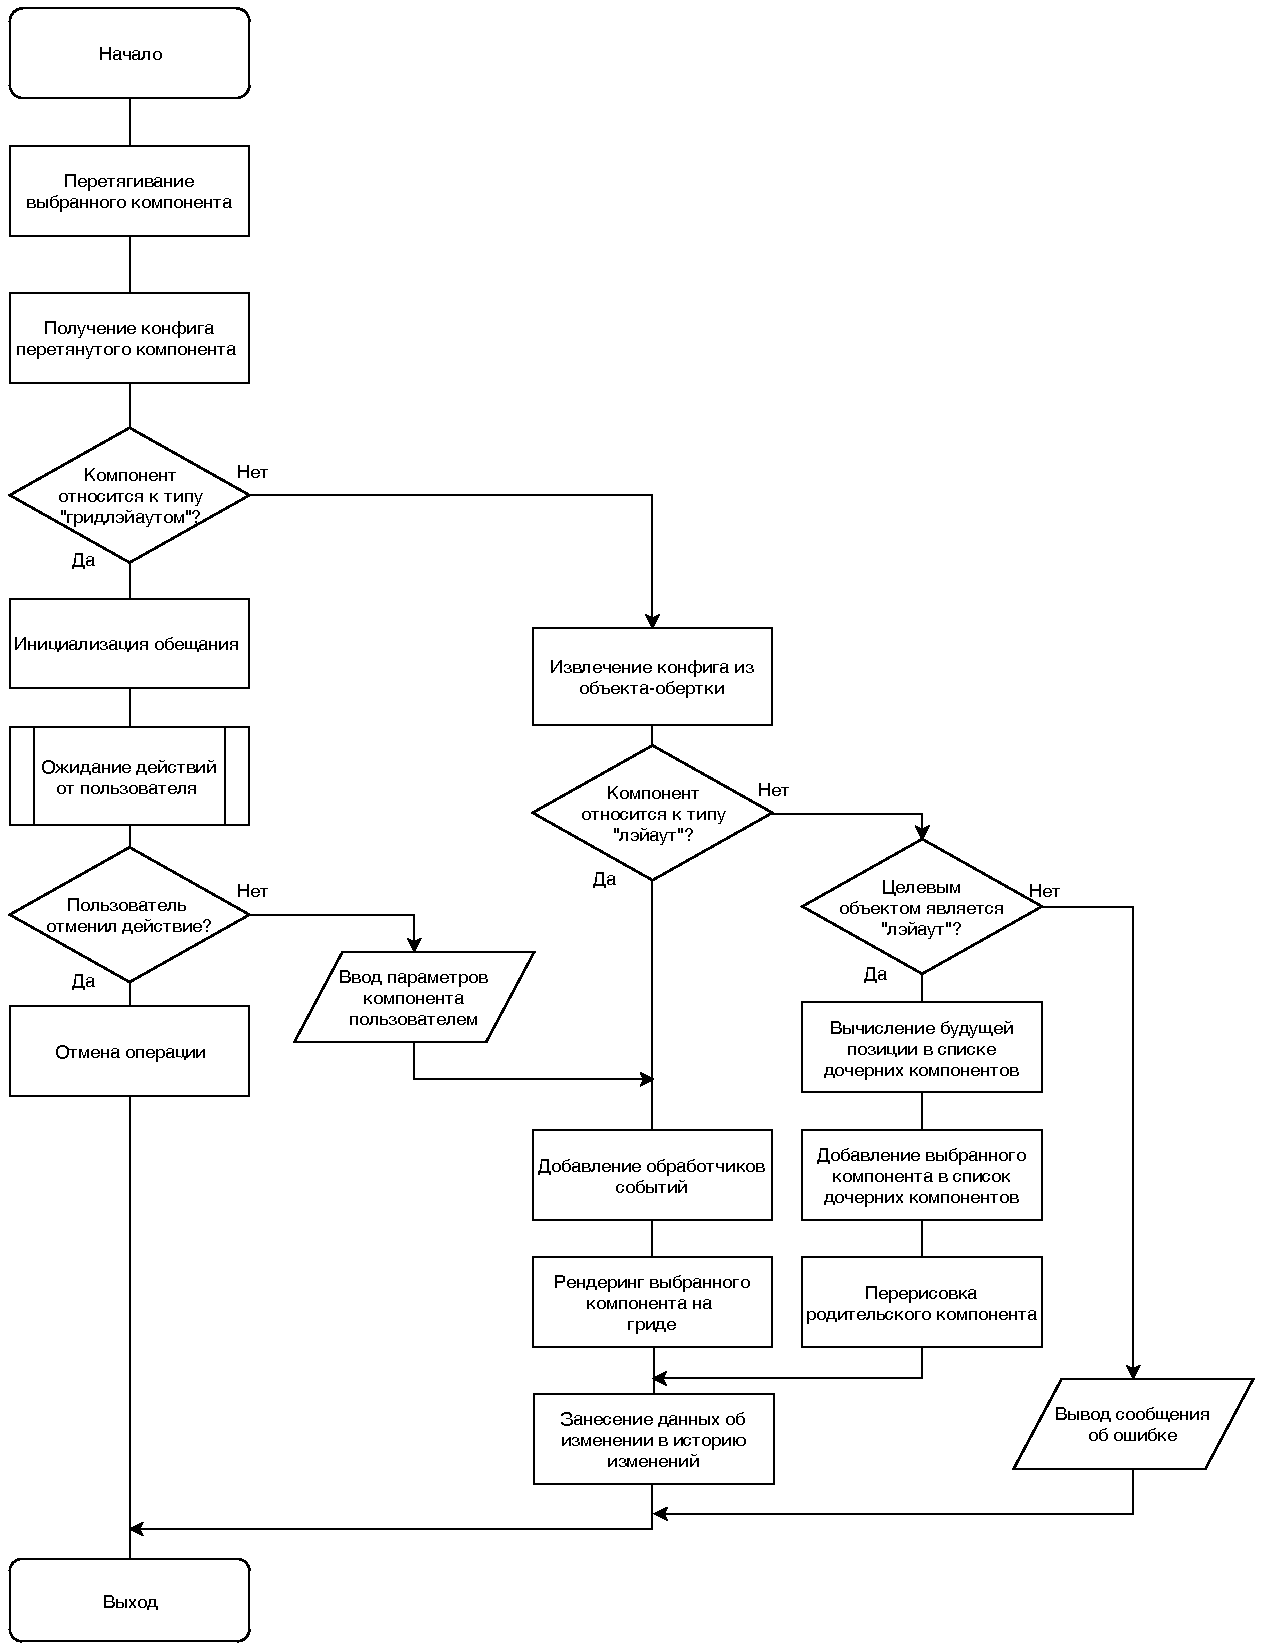
\includegraphics[scale=0.65]{composition.pdf}
    \caption{Алгоритм компоновки графических компонентов}
    \label{sec:dev:composition}
\end{figure}
\subsection{Разработка инспектора свойств}
\label{sec:development:property_inspector}

Инспектор свойств является панелью, содержащей множество вкладок, поэтому были использованы такие базовые графические компоненты, предоставляемые библиотекой Webix, как:

\begin{itemize}
    \item TabView - для дозирования количества одновременно отображаемой информации путем предоставления доступа к ее частям посредством разделения на страницы;
    \item Accordion - для группирования отображаемой информации в логически или технически обусловленные группы свойств.
\end{itemize}

Конфиг компонента представляет собой набор <<страниц>>, реализованный посредством компонента TabView. Каждая страница содержит в себе компонент Accordion, позволяющий манипулировать отображением собственного содержимого.

\begin{lstlisting}
this.addView({
  rows: [
    undoRedoConfig,
    { ...getSearchPanel() },
    {
      id: webix.uid(),
      borderless: true,
      view: 'tabview',
      cells: [
        {
          header: 'Data',
          ...getAccDataConfig()
        }
        {
          header: 'Style',
          ...getAccStyleConfig(this)
        }
        {
          header: 'Code',
          ...getElementCodeConfig()
        }
      ]
    }
  ]
})
\end{lstlisting}

Компонент Accordion, использующийся с целью отображения свойств выделенных компонентов, в свою очередь использует специальный компонент библиотеки Webix, называющийся <<property>>, который был специально создан для подобных целей.

Метод onAfterEditStop вызывается по окончании пользователем ввода данных в поле свойства. Здесь осуществляются проверки введенных данных на валидность и их дальнейшая обработка.

На случай ввода неверных данных предусмотрены дополнительные обработчики и средства вывода информации, с целью уведомить пользователя об ошибке.

\begin{lstlisting}
{
  id: getSettingsId(),
  view: 'property',
  onContext: {},
  elements: getElements(),
  autoheight: true,
  nameWidth: 120,
  on: {
    onAfterEditStop(state, editor): void {
      if (Number.isInteger(Number(state.value))) {
        state.value = Number(state.value);
      }

      if (Number(state.value) !== state.old) {
        let view = <any>this.getTopParentView()
          .getLastActiveComponent();

        if (view) {
          if (editor.id === 'url') {
            view.clearAll();
            view.config.data = null;
          } else if (editor.id === 'top' || editor.id === 'left') {
            view.getParentView().config[editor.id] = state.value;
            view.getParentView()
                .resize();
          }

          // visible component editing
          view.config[editor.id] = state.value;

          if (view.setTemplate) {
            view.setTemplate();
          }
          if (view.refresh) {
            view.refresh();
          }

          view.resize();
          view.callEvent('onBlur');
          view.callEvent('onFocus', [view]);
        } else {
          webix.message({
            text: 'Attempt to change property of not existing item',
            type: 'error',
            expire: 2000
          });
        }
      }
    }
  }
}
\end{lstlisting}

Основным инструментом для работы с компонентами является панель свойств, отображающая свойства выделенного компонента.

\begin{lstlisting}
definePropertyTable(viewConfig) {
  let elements = [];
  let propertyTable = this.$$(getSettingsId());

  this.$$(getAccStyleId()).config.data = viewConfig;

  const elementCodeView = this.$$(getElementCodeId());

  if (viewConfig) {
      if (viewConfig.view === 'datatable') {
          elements = getDatatableElements();
      } else {
        Object.entries(viewConfig)
          .forEach(([key]) => {
            if (
              key === 'id'
              || key === '_inner'
              || key === 'template'
            ) {
              return;
            }

            let type = 'text';
            if (key.search(/color/gi) !== -1) {
              type = 'color';
            }

            elements.push({
              id: key,
              label: key,
              type
            });
        });
      }
  }

  elementCodeView.setValue(`${getPrettyJson(viewConfig)}`);
  elementCodeView.refresh();

  propertyTable.define('elements', elements);

  let parsedItem = getParsedConfig(viewConfig);

  propertyTable.setValues(parsedItem);

  propertyTable.resize();
}
\end{lstlisting}

Чтобы после выделения пользователем компонента его свойства отображались во вкладке свойства инспектора свойств необходимо было добавить в его метод инициализации соовтествующий обработчик события.

\begin{lstlisting}
() => {
  if (!this.config.gridId) { return; }
  eventHandlerInit(this.config.gridId);
  const grid = $$(this.config.gridId);

  grid.attachEvent('onMovableElementSelect', target) =>{
    focusEventHandler(target);
    this.setLastActiveComponent(target);
    let configCopy = null;

    try {
      configCopy = webix.copy(target.config);
    } catch (e) {
      configCopy = webix.clone(target.config);
    }
    this.definePropertyTable(configCopy);

    if (target.config.view === 'datatable') {
      showColumnsForm(this, target);
    } else {
      hideColumnsForm(this);
    }
  });
}
\end{lstlisting}

При срабатывании события onMovableElementSelect происходит копирование свойств компонента с помощью метода библиотеки. Функции showColumnsForm и hideColumnsForm отвечают за управление отображением дополнительной вкладки свойств, доступной лишь после выделения особого компонента, предоставляемого библиотекой Webix, нужнающегося в дополнительной конфигурации - Datatable.

Данная особенность обусловлена особой струкурой компонента и соответсвующего ему DOM-элемента.

Помимо всего вышеперечисленного, инспектор свойств предоставляет возможность поиска свойства как по ключу, так и по значению, что значительно упрощает работу с комплексными компонентами, содержащими большое количесво свойств.

Для этого в самом верху инспектора свойств расположена панель ввода с соовтествующей иконкой.

Далее будет представлен код, описывающий логику данного компонента.

\begin{lstlisting}
const tabviewSearch = {
  id: getSearchPanelId(),
  view: 'search',
  hotkey: 'enter',
  placeholder: 'Search any property',
  on: {
    onChange() {
      getInputValue.call(this);
    },
    onFocus() {
      // blocking events in order to prevent starting search
      this.blockEvent();
      this.getNode().children[0].children[0].select();
      this.unblockEvent();
    },
    onEnter() {
      getInputValue.call(this);
    }
  }
};
\end{lstlisting}

Секция on содержит обработчики одноименных событий. Свойство hotkey указывает горячую клавишу для вызова события onEnter, которое осуществляет вызов функции getInputValue с контектом объекта компонента поиска.

Функция getInputValue инкапсулирует функциональность поиска данных по ключу и значению. Ее код преставлен ниже.

\begin{lstlisting}
function getInputValue(): void {
  const list = <webix.ui.list>this.getTopParentView().$$(getSearchListId());
  const val: string = this.getTopParentView().$$(getSearchPanelId()).getValue().toLowerCase()
    .trim();
  const store: object = getParsedConfig(this.getTopParentView().$$(getAccStyleId()).config.data);

  list.clearAll();

  if (store && val) {
    this.getTopParentView().$$(getSearchListId()).clearAll();

    Object.entries(store).forEach(([key, value]) => {
      if (JSON.stringify(value) !== undefined
        && (key.toLowerCase().indexOf(val) !== -1
          || JSON.stringify(value).indexOf(val) !== -1)
      ) {
        if (typeof value === 'string') {
          value = value.trim();
        }
        list.parse({ key, value }, '');
      }
    });
  }

  this.blur();
  list.getParentView().getParentView().show();
  list.getParentView().define({ collapsed: false });
  list.getParentView().refresh();
}
\end{lstlisting}

По окончании выполнения вышеуказанных в функции getInputValue действий, все найденные свойства добавятся в содержимое компонента, отображающего результаты поиска в виде списка. Вкладка с результатами поиска будет открыта автоматически, что определенно благоприятно скажется на UX.

Функциональность самого списка результатов поиска не ограничивается одним лишь отображением самих результатов поиска - при нажатии на один из отображаемых результатов система автоматически отобразит пользователю нужную вкладку и, более того, сразу откроет поле с искомым свойтсвом в режиме редактирования.

Ниже будет предоставлен фрагмент кода с конфигом данного компонента, где будут видны некоторые детали реализации.

\begin{lstlisting}
const searchListId = 'AC:settings:searchList';

const getSearchListId = (): string => searchListId;

const searchListConfig = {
  id: getSearchListId(),
  template: '{#key#: #value#}',
  select: true,
  view: 'list',
  on: {
    onItemClick(itemId): void {
      const accordion = this.getTopParentView().$$(getScrollViewId()).getParentView().getParentView();
      accordion.define('collapsed', false);

      let key = this.getItem(itemId).key;

      if (key !== 'id') {
        this.getTopParentView().$$(getSettingsId()).edit(this.getItem(itemId).key);
      }
    }
  },
  data: []
}
\end{lstlisting}

Подобная реализация также определенно благоприятно скажется на UX, ведь в перспективе пользователю необходимо будет совершать значительно меньше действий для достижения желаемого.
